\documentclass[14pt,t,aspectratio=169]{beamer}
\usepackage{fontspec}
\usepackage{color}
\usepackage{minted}
\usepackage{array}
\usepackage{emoji}

%% These fonts are non-free.
%% Comment out the lines if you don't have them.
\setmainfont{Equity Text A}
\setsansfont{Concourse T3}
\setmonofont{Triplicate T4}

\definecolor{bgcolor}{RGB}{255,240,240}
\definecolor{red}{RGB}{224,35,35}
\setbeamercolor{background canvas}{bg=bgcolor}
\setbeamercolor{normal text}{fg=black}
\setbeamercolor{titlelike}{fg=black}
\setbeamercolor{itemize item}{fg=red}
\setbeamercolor{enumerate item}{fg=red}
\setbeamertemplate{itemize items}[circle]
\setbeamertemplate{navigation symbols}{}
\usemintedstyle{monokai}
\newminted[lispcode]{common-lisp}{fontsize=\footnotesize}
\newminted[smalllispcode]{common-lisp}{fontsize=\scriptsize}
\def\code#1{{\color{codecolor}\texttt{#1}}}
\renewcommand{\theFancyVerbLine}{\color{darkgray}\large \oldstylenums{\arabic{FancyVerbLine}}}

\usebackgroundtemplate{
\includegraphics[width=\paperwidth,height=\paperheight]{background}}
\begin{document}
{\usebackgroundtemplate{
\includegraphics[width=\paperwidth,height=\paperheight]{firstpage}}
  \begin{frame}
    \color{white}
    \vspace{3cm}
    {\hspace{1.4cm} \LARGE Porting SBCL to the Nintendo Switch} \\
    \vspace{1cm}
    {\hspace{1.6cm} Yukari Hafner, Charles Zhang} \\
    \vspace{0.2cm}
    {\hspace{2.1cm}\texttt https://shirakumo.org}
  \end{frame}}

\begin{frame}
  \frametitle{The Device}
  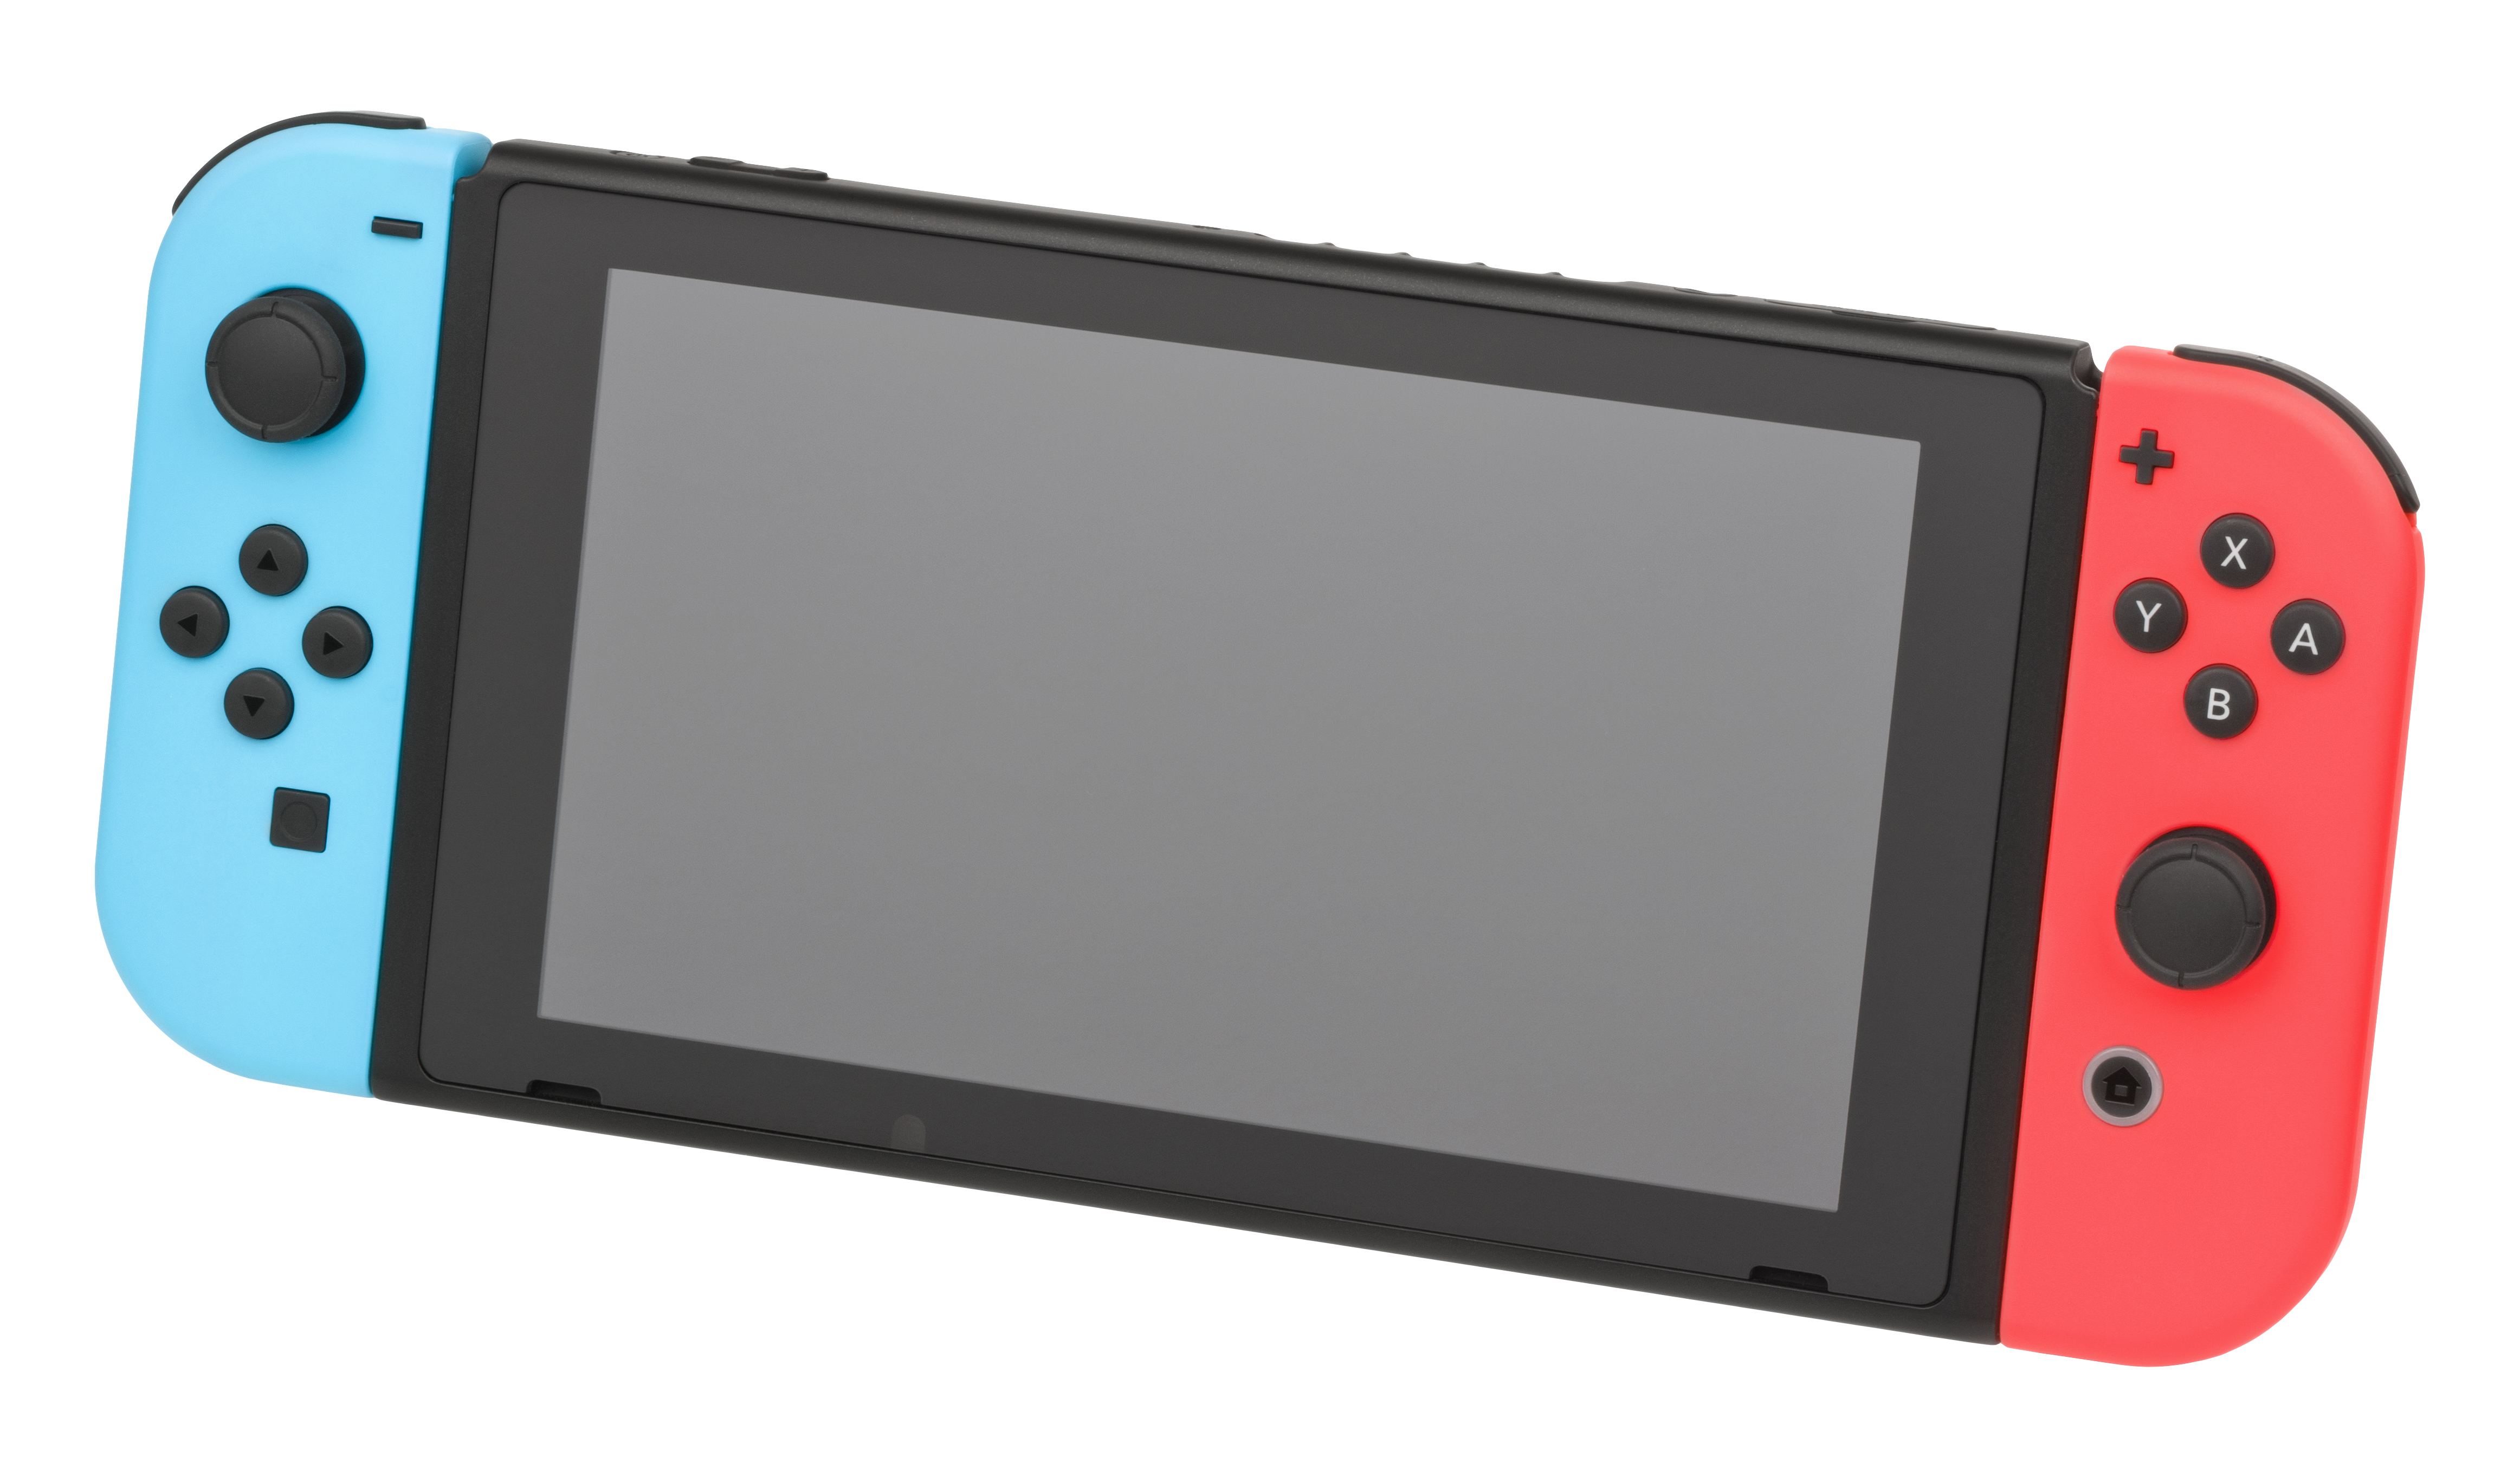
\includegraphics[height=5cm]{switch}
  \begin{itemize}
  \item CPU: ARM 4 Cortex-A57 64-bit
  \item OS: ``Horizon OS'', proprietary micro-kernel
  \item SDK: C++, proprietary version of Clang
  \end{itemize}
\end{frame}

\begin{frame}
  \frametitle{Immediate Challenges}
  \begin{itemize}
  \item Everything is proprietary and under NDA \\
    \Rightarrow{} Scarce public information
  \item The OS is not BSD or even fully POSIX \\
    \Rightarrow{} Need new OS abstractions
  \item There are no inter-thread signals \\
    \Rightarrow{} Can't use usual GC tricks
  \item We are not allowed to create executable pages \\
    \Rightarrow{} No compilation at runtime
  \end{itemize}
\end{frame}

\begin{frame}
  \frametitle{Basic Ideas}
  \begin{itemize}
    \color{lightgray}
  \item Everything is proprietary and under NDA \\
    \textcolor{red}{\Rightarrow} \textcolor{black}{Only publicise our own interfaces}
  \item The OS is not BSD or even fully POSIX \\
    \textcolor{red}{\Rightarrow} \textcolor{black}{Write C(++) shim libraries for access}
  \item There are no inter-thread signals \\
    \textcolor{red}{\Rightarrow} \textcolor{black}{Use safepoints}
  \item We are not allowed to create executable pages \\
    \textcolor{red}{\Rightarrow} \textcolor{black}{Compile everything on linux and shrinkwrap}
  \end{itemize}
\end{frame}

\begin{frame}
  \frametitle{A Standard SBCL Build}
  \begin{itemize}
  \item build-config \\
    \Rightarrow{} Gather system info
  \item make-host-1 \\
    \Rightarrow{} Emit C headers and support files
  \item make-target-1 \\
    \Rightarrow{} Compile the C runtime on the target
  \item make-host-2 \\
    \Rightarrow{} Cross-compile the compiler on the host
  \item make-target-2 \\
    \Rightarrow{} Use the compiler from the host to\\ incrementally compile the rest on the target
  \end{itemize}
\end{frame}

\begin{frame}
  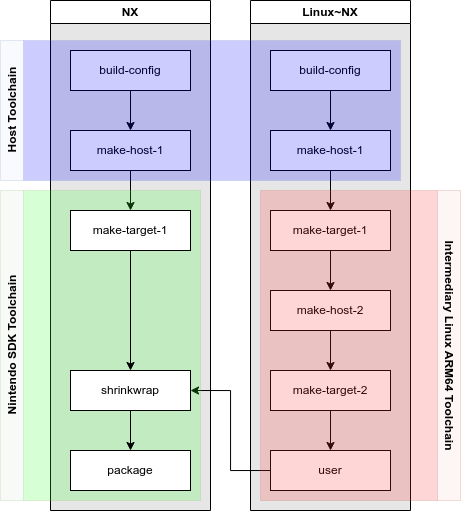
\includegraphics[height=8.5cm]{build.png}
\end{frame}

\begin{frame}
  \frametitle{Relocation}
  \begin{itemize}
  \item 
  \end{itemize}
\end{frame}

\begin{frame}
  \frametitle{Garbage Collection}
  \begin{itemize}
  \item 
  \end{itemize}
\end{frame}


\begin{frame}[c]{ }
  \centering
  {\Huge Live Demo}
\end{frame}

\begin{frame}
  \frametitle{Further Work}
  \begin{itemize}
  \item Optimising CLOS dispatch ahead of time \\
    \Rightarrow{} Christophe? \emoji{pleading-face}
  \item Optimising Trial and Kandria \\
    \Rightarrow{} Lots of profiling work that can be done on PC
  \item Porting to the Nintendo Switch 2 \\
    \Rightarrow{} As soon as plebians like us get access from almighty \\\quad Nintendo
  \end{itemize}
\end{frame}

{\usebackgroundtemplate{
\includegraphics[width=\paperwidth,height=\paperheight]{firstpage}}
  \begin{frame}[c]{ }
    \centering\color{white}
    \vspace{2cm}
    {\LARGE Thank you!} \\
    \vspace{0.2cm}
    Consider supporting our work: \\
    
\includegraphics[width=3cm]{patreon} \\
    {\texttt https://patreon.com/shinmera}
  \end{frame}}
\end{document}

%%% Local Variables:
%%% mode: latex
%%% TeX-master: t
%%% TeX-engine: luatex
%%% TeX-command-extra-options: "-shell-escape"
%%% End:
